\begin{center}
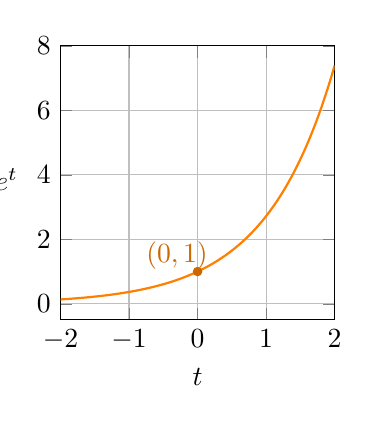
\begin{tikzpicture}
\begin{axis}[
    width=\dimexpr0.5\linewidth-1cm\relax,
    height=\dimexpr0.5\linewidth-1cm\relax,
    grid=both,
    unbounded coords=jump,
    title style={font=\small, yshift=0.6em},
    xlabel=$t$,
    ylabel style={%
        rotate=-90,
        anchor=east,
        overlay%
    },
    ylabel={$\varphi(t)=e^t$},
    xmin=-2, xmax=2,
    ymin=-0.5, ymax=8
]
\addplot[orange,thick,domain=-2:2,samples=200]{exp(x)};
\addplot[only marks, mark=*, mark size=1.5pt, orange!80!black] coordinates {(0,1)};
\node[orange!80!black] at (axis cs:-0.3,1.5) {$(0,1)$};
\end{axis}
\end{tikzpicture}
\end{center}